\documentclass{beamer}
\renewcommand\thesection{\arabic{section}}
\newcommand{\myfont}{\rmfamily\normalsize\upshape\mdseries}
\newcommand{\degree}{^\circ}
\title{\sffamily Answer for RC3}

\institute[UM-SJTU JI]{University of Michigan-Shanghai Jiao Tong University Joint Institute}
\author{HamHam}
\usepackage{graphicx}
\usepackage{picinpar}
\usepackage{indentfirst}
\usepackage{chemformula}
\usepackage{geometry}
\usepackage{subfigure}
\usepackage{appendix}
\usepackage{amsfonts,amsmath,amssymb}
\usepackage{enumerate}
\usepackage{float}
\usepackage{geometry}
\usepackage{latexsym}
\usepackage{listings}
\usepackage{multicol,multirow,multido}
\usepackage{tabularx}
\usepackage{ulem}
\usepackage{tikz}
\usepackage{xcolor}
\usepackage{cite}
\usepackage{setspace}
\usepackage{hyperref}
\usepackage{textpos}
\usepackage{booktabs}

\usetheme[dove]{Boadilla}
\usecolortheme{dolphin}
\useoutertheme{miniframes}
\begin{document}
    \usebackgroundtemplate{\tikz\node[opacity=0.3]{
    
\includegraphics[width=\paperwidth,
    height=\paperheight]{hamster.jpg}
    };}
\begin{titlepage}
    \begin{center}
        VV186 - Honors Mathmatics II
    \end{center}
\end{titlepage}
\myfont

    \begin{frame}
        \frametitle{Exercise}
        2. Prove that $\lim_{n\rightarrow \infty} \sqrt[n]{n}=1$.\\ 
        \vspace{3em}
        Some results:
        \begin{itemize}
            \item $\lim_{n\rightarrow \infty} \sqrt[n]{a}=1,a>0$
            \item $\lim_{n\rightarrow \infty} \frac{1}{n^\alpha}=0,\alpha\in (0,+\infty)$
        \end{itemize}
    \end{frame}
    \begin{frame}
        \frametitle{Solution}
    2.\\
    \hspace{1em} We consider the case for $n\geq 2$. Since $\sqrt[n]{n}>1$ for all $n\geq 2$, we can choose a 
    non-negative sequence, let say $(b_n)_{n\geq 2}$ such that
    \begin{equation*}
        1+b_n=\sqrt[n]{n}
    \end{equation*}
    \hspace{1em} From the fact that 
    \begin{equation*}
        (1+b_n)^n=\sum^n_{k=0}\left(\begin{smallmatrix}n\\k\end{smallmatrix}\right)1^k\cdot b_n^{n-k}
    \end{equation*}
    and another fact that $(1+b_n)^n=n$, we get the following inequality
    \begin{equation*}
        n=(1+b_n)^n\geq \left(\begin{smallmatrix}n \\ 2\end{smallmatrix}\right) b^2_n=\frac{n(n-1)}{2}b^2_n
    \end{equation*}
    \end{frame}
    
    \begin{frame}
        \frametitle{Solution}
    2.$(continue)$\\
    \hspace{1em} After some algebraic works, one can see 
    \begin{equation*}
        b_n\leq\sqrt{\frac{2}{n-1}}
    \end{equation*}
    \hspace{1em} But this means 
    \begin{equation*}
        0\leq \sqrt[n]{n}-1\leq \sqrt{\frac{2}{n-1}}
    \end{equation*}
    \hspace{1em} By taking the limit, we have
    \begin{equation*}
        0\leq \lim_{n\rightarrow\infty}(\sqrt[n]{n}-1)\leq \lim_{n\rightarrow\infty}\sqrt{\frac{2}{n-1}}=0
    \end{equation*}
    \end{frame}
    
    \begin{frame}
        \frametitle{Solution}
    2.$(continue)$\\
    \hspace{1em} Finally, by Squeeze theorem, we get 
    \begin{equation*}
        \lim_{n\rightarrow\infty}(\sqrt[n]{n}-1)=\lim_{n\rightarrow\infty}\sqrt[n]{n}-1=0
    \end{equation*}
    \hspace{1em} We conclude
    \begin{equation*}
        \lim_{n\rightarrow\infty}\sqrt[n]{n}=1\quad\square
    \end{equation*}
    \end{frame}



    \begin{frame}
        \frametitle{Exercise}
        3. A sequence is defined as
        \begin{equation*}
            (S_n)_{n\in\mathbb{N}}, S_1=\sqrt{2}, S_2=\sqrt{2+\sqrt{2}}, S_3=\sqrt{2+\sqrt{2+\sqrt{2}}},...
        \end{equation*}
        Please prove that it is convergent and calculate the limit of $(S_n)$ as $n\rightarrow \infty$.
    \end{frame}
    
        \begin{frame}
            \frametitle{Solution}
            3.\\
            \hspace{1em}Obviously $S_n$ is increasing, now we use
            induction to prove that $S_n$ is bounded. Let $A(n) :S_n < 2$.\\
            \hspace{1em}\textcolor{red}{Base case:} $S_1=\sqrt{2}<2$, so $A(1)$ is valid.\\
            \hspace{1em}\textcolor{red}{Inductive case:} Suppose that $A(n)$ is true, namely $S_n < 2$, we have $S_{n+1}=\sqrt{2+S_n}<\sqrt{2+2}=2$, 
            therefore $A(n+1)$ is true.\\
            \vspace{0.5em}
            Since $S_n$ is monotonic and bounded, so it converges, say $\lim_{n\to \infty} S_n = s$. Considering the recursive definition
            
            $$S_{n+1}^2=S_n+2$$,
            we take the limit from both side and get $s^2=2+s$. Since $s$ should be positive, so $s=2$. And we conclude
            $$\underset{n\to \infty}{\lim}\sqrt{2+\sqrt{2+\dots+\sqrt{2}}}=2$$
        \end{frame}

        \begin{frame}
            \frametitle{Exercise}
            4. Prove that every Cauchy sequence has at most one accumulation point.
            (A Former Midterm Question)
            
            \vspace{2em}
            Tips:
            \begin{itemize}
                \item You should work on an abstract metric space, using $\rho $ instead of $| \cdot |$.
                \item Try to prove this without using proof by contradiction!
            \end{itemize}
        \end{frame}
    \begin{frame}
        \frametitle{Solution}
        4.\\
        \textbf{Proof:} Let $\left < x_n \right >$ be such a sequence and let $\left < x_{n_k} \right >$, $\left < x_{n_j} \right >$ be two subsequences of it with different limits $a$, $b$. 
        Let $\varepsilon = \frac{1}{3} \rho(a, b)$. For any $N \in \mathbb{N}$, choose some $n_k > N$ and $n_j > N$, 
        such that $\rho(x_{n_k}, a) < \varepsilon$ and $\rho(x_{n_j}, b) < \varepsilon$. If $\rho(x_{n_k}, x_{n_j}) < \varepsilon$ then 
    \begin{equation*}
        \rho(a, b) \leq \rho(a, x_{n_k}) + \rho(x_{n_k}, x_{n_j}) + \rho(x_{n_j}, b) < 3 \varepsilon = \rho(a, b),  
    \end{equation*} 
    which implies that $\rho(a, b) < 0$, a contradiction. 
        
    \vspace{2em}
    Without using proof by contradiction: try to prove $a=b$.
    \end{frame}
    \begin{frame}
        \frametitle{Exercise}
        5. Let ($a_n$) be a real sequence that converges to $L \in \mathbb{R}$.
        Prove that the sequence ($\frac{\sum_{i=1}^n a_i}{n}$) is convergent. 
        Furthermore $\underset{n\rightarrow \infty}{\lim} (\frac{\sum_{i=1}^n a_i}{n})=L $.
    \end{frame}
    \begin{frame}
        \frametitle{Solution}
        \centering
        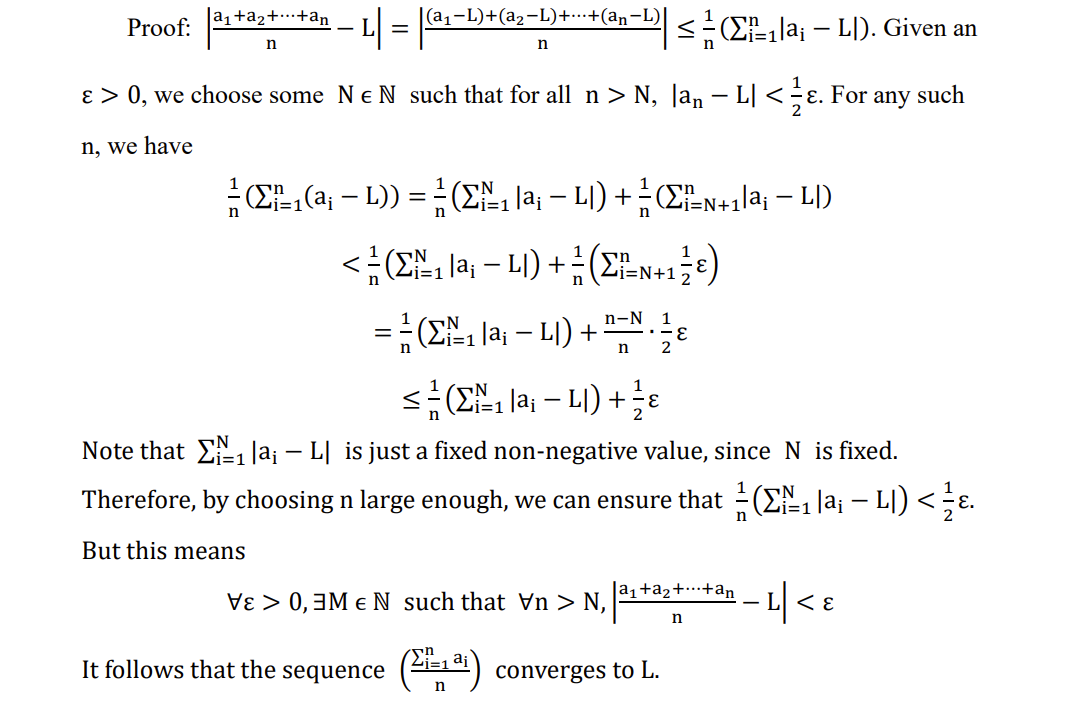
\includegraphics[height=0.8\textheight]{sol_4.png}
        
    \end{frame}
    
     \begin{frame}
        \frametitle{Exercise}
    6. Let $(a_n),(b_n)$ be two real sequences. Furthermore, assume that $a_n<b_n$
    for all $n$, $[a_{n+1}, b_{n+1}]\subseteq [a_n,b_n]$, $\lim (a_n-b_n)=0$. Prove that there 
    is an unique $m\in [a_n,b_n]$ for all $n$, such that 
    \begin{equation*}
        \lim a_n=\lim b_n=m
    \end{equation*}
    \end{frame}
    \begin{frame}
        \frametitle{Solution}
    6.\\
    $Proof$ : \\
    \hspace{1em} We first show that $(a_n),(b_n)$ are convergent. Notice that $[a_{n+1}, b_{n+1}]\subseteq [a_n,b_n]$ 
    means that $(a_n)$ is increasing, while $(b_n)$ is decreasing. Furthermore, both $(a_n)$ and $(b_n)$ are bounded by 
    $[a_0,b_0]$. Therefore, $(a_n)$ and $(b_n)$ are convergent.\\
    \hspace{1em} Next we show that $\lim a_n=\lim b_n$. Suppose $\lim b_n=L$, where $L$ is a unique number since a sequence 
    has precisely one limit. Then we know 
    \begin{equation*}
        \lim a_n=\lim [(a_n-b_n)+b_n]=\lim (a_n-b_n) + \lim b_n= 0+L=L
    \end{equation*}
    Moreover, since 
    $\begin{cases}
        L \geq a_n\\
        L \leq b_n
    \end{cases}$, we know that $L\in [a_n,b_n]$.$\quad\square$
    
    \end{frame}
    \begin{frame}
        \frametitle{Exercise}
        7. Let ($a_n$) be a sequence that $a_n=\frac{1}{\sqrt{n^2+1}}+\cdots+\frac{1}{\sqrt{n^2+n}}$.
        Calculate the limit of ($a_n$).    
    
    \end{frame}
    
\begin{frame}
    \frametitle{Solution}
7.\\
\hspace{1em} We first consider two sequence $(b_n)_{n\geq 1},(c_n)_{n\geq 1}$ given by 
\begin{equation*}
    \begin{cases}
        b_n:=\frac{1}{\sqrt{n^2}}+\dots+\frac{1}{\sqrt{n^2}}\\
        c_n:=\frac{1}{\sqrt{n^2+n}}+\dots+\frac{1}{\sqrt{n^2+n}}
    \end{cases}
\end{equation*}
\hspace{1em} Clearly, 
$\begin{cases}
    (b_n)\leq (a_n)\\
    (c_n)\geq (a_n)
\end{cases}$ 
for all $n\geq 1$. \\
\hspace{1em} Then one can easily find out the limit for both $(b_n)$ and $(c_n)$, which can be calculated as 
\begin{equation*}
    \lim_{n\rightarrow\infty}b_n=\lim_{n\rightarrow \infty}\sum^n_{k=1}\frac{1}{\sqrt{n^2}}=\lim_{n\rightarrow \infty}\sum^n_{k=1}\frac{1}{n}=\lim_{n\rightarrow\infty}\frac{n}{n}=\lim_{n\rightarrow\infty}1=1
\end{equation*}
\end{frame}

\begin{frame}
    \frametitle{Solution}
7.$(continue)$\\
\begin{equation*}
    \lim_{n\rightarrow\infty}c_n=\lim_{n\rightarrow \infty}\sum^n_{k=1}\frac{1}{\sqrt{n^2+n}}=\lim_{n\rightarrow \infty}\frac{n}{\sqrt{n^2+n}}=\lim_{n\rightarrow\infty}\frac{1}{\sqrt{1+\frac{1}{n}}}=1
\end{equation*}
\hspace{1em} By Squeeze Theorem, we know 
\begin{equation*}
    \lim_{n\rightarrow\infty}b_n\leq \lim_{n\rightarrow\infty}a_n\leq \lim_{n\rightarrow\infty}c_n
\end{equation*}
, namely
\begin{equation*}
    1\leq \lim_{n\rightarrow\infty}a_n\leq1
\end{equation*}
We conclude that $ \lim_{n\rightarrow\infty}a_n=1\quad\square$
\end{frame}

\end{document}